Tato kapitola se zaměřuje na analýzu problémové domény. Obsahuje její struč\-ný popis, analýzu procesů, které souvisejí s vedením třídních knih, a návrh na zlepšení či optimalizaci identifikovaných procesů. Dále obsahuje doménový model, který pomůže s vizualizací objektů z reálného světa, popíše jednotlivé entity a přiblíží vztahy mezi nimi. Výsledkem analýzy jsou funkční a nefunkční požadavky, které jsou kladeny na vznikající informační systém.

Veškeré modely obsažené v této kapitole jsou vytvářeny s pomocí jazyka UML a programu Enterprise Architect.

\section{Popis problematiky školní dokumentace}
Problémovou doménou je vedení školní dokumentace, konkrétně vedení třídních knih. Bližší informace o vedení povinné dokumentace škol a školských zařízeních můžeme najít ve Školském zákoně č. 561/2004 Sb., o předškolním, základním, středním, vyšším odborném a jiném vzdělávání v § 28 č. 1 \cite{zk561}.

Zákon stanovuje, že školy a školská zařízení jsou povinny vést mimo jiné i třídní knihu, která obsahuje průkazné informace o poskytovaném vzdělání a jeho průběhu. Informace o obsahové stránce či struktuře dokumentu nejsou zákonem ani žádným jiným předpisem blíže specifikovány. \cite{zk561}

\subsection{Archivace}
Ať už škola vede dokumenty v papírové nebo elektronické podobě, musí se při archivaci řídit zákonem č. 499/2004 Sb., o archivnictví a spisové službě a o změně některých zákonů \cite{zk499}. Ten v § 2 písm. e) říká, že \uv{\textit{dokumentem je každá písemná, obrazová, zvuková nebo jiná zaznamenaná informace, ať již v podobě analogové či digitální}}.

U dokumentů uchovávaných v digitální podobě musí být podle § 3 odst. 5 zákona č. 499/2004 Sb. zajištěna věrohodnost původu dokumentů a neporušitelnost jejich obsahu a čitelnosti. K tomuto účelu lze použít například elektronický podpis nebo elektronické časové razítko \cite{zk499}.

Zákon dále udává dokumenty, které se řadí do archiválií. Příloha č. 2 k zákonu č. 499/2004 Sb., bod 16 říká, že mezi dokumenty, které se řadí mezi archiválie patří \uv{\textit{třídní výkazy, katalogy, katalogové listy, protokoly o závěrečných zkouškách, protokoly o maturitních zkouškách vydané základními a středními školami a protokoly o státních závěrečných zkouškách na vysokých školách}}.

\subsection{GDPR}
GDPR neboli General Data Protection Regulation je Obecné nařízení na ochranu osobních údajů, které je účinné v zemích EU od 25. května 2018. Jedná se o nařízení Evropské unie, jehož cílem je zvýšit ochranu osobních údajů Evropanů. \cite{uoou-gdpr}

GDPR definuje osobní údaje jako veškeré informace vztahující se k identifikované či identifikovatelné fyzické osobě. Mezi obecné osobní údaje nařízení řadí například jméno, příjmení, datum narození, fotografický záznam, IP adresu nebo telefonní číslo. Ve školním prostředí mohou být za osobní údaje považovány záznamy o chování, známky a vysvědčení. Citlivé údaje jsou podle GDPR speciální kategorií osobních údajů. Mezi citlivé údaje patří například informace o rasovém či etnickém původu, zdravotním stavu nebo náboženském vyznání. Zpracování těchto údajů podléhá přísnějším opatřením než je tomu u obecných osobních údajů. \cite{uoou-prirucka, gdpr-pro-ucitele}

GDPR se týká každého, kdo shromažďuje nebo zpracovává osobní údaje obyvatelů Evropské unie. Nařízení se tedy týká i škol, které se jím musejí řídit. Školy typicky musejí spravovat osobní údaje o dětech, k tomu je v některých případech potřeba souhlas zákonných zástupců. Dále mohou spravovat citlivé údaje, kombinaci osobních údajů více subjektů, apod. Aby se škola vyhnula velkým pokutám, které hrozí za porušení nařízení, musí škola identifikovat, jaká data bude zpracovávat a jaký je k tomu právní důvod. Dále musí nastavit procesy tak, aby zajistila bezpečnost dat při práci a uchovávání. Nařízení také ukládá škole povinnost zavést pozici Pověřence pro ochranu osobních údajů.~\cite{gdpr-ve-skolstvi}

S GDPR souvisí zákon č. 110/2019 Sb. o zpracování osobních údajů. Tento zákon upřesňuje práva a povinnosti, které vyplývají z Obecného nařízení o ochraně osobních údajů. \cite{epravo-osobni-udaje}


\section{Procesy}
Tato podkapitola je věnována identifikaci klíčových procesů v problémové doméně. Každý proces bude popsán z pohledu současného stavu, tedy bez použití informačního systému, a z pohledu stavu budoucího, tedy s použitím informačního systému pro správu třídních knih. Ve vybrané doméně byly identifikovány následující klíčové procesy.

\subsection{Zápis o proběhnuté hodině do třídní knihy}
\subsubsection*{Bez použití informačního systému}
Předpokladem pro tento proces je, že má učitel u sebe třídní knihu. To však nemusí být vždy pravda. Třídní kniha může být při přesunu žáků zapomenuta v jiné učebně, než právě probíhá výuka. Pokud toto nastane, učitel musí třídní knihu nejprve nalézt.

Proces je jinak velice přímočarý. Učitel nejprve vezme třídní knihu, nalistuje v ní potřebnou stranu, na kterou zápis patří, zjistí informace a zapíše je. Informace, které se typicky zapisují, jsou absence, předmět, probírané téma a podpis. Namodelovaný proces lze vidět na obrázku \ref{zapis_bez_IS}.

\begin{figure}[h]
	\centering
	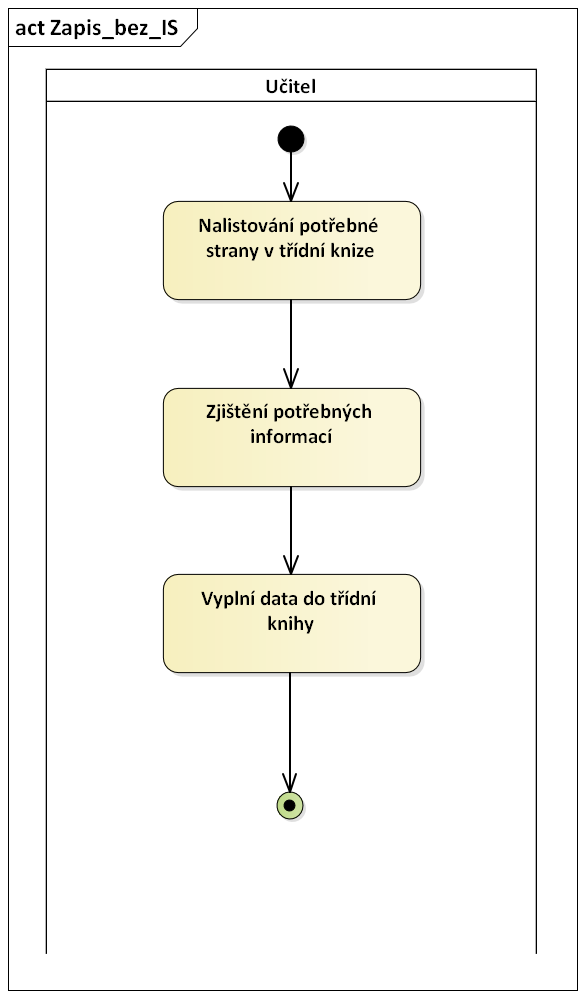
\includegraphics[width=0.5\textwidth]{images/Zapis_bez_IS.png}
	\caption{Proces zápisu o proběhnuté hodině bez informačního systému}
	\label{zapis_bez_IS}
\end{figure}

\subsubsection*{S použitím informačního systému}
S použitím informačního systému odpadá problém s hledáním zapomenuté třídní knihy. Další výhodou použití informačního systému také je přístup odkudkoliv, který pomáhá řešit problémy s třídní knihou vzniklé při distanční výuce.

Proces je stejně přímočarý, jako bez použití informačního systému. Učitel se nejdříve přihlásí do systému, vybere v aplikaci třídní knihu, do které chce zapisovat, zjistí informace a vyplní je. Vyplňovaná data jsou stejná, jako bez použití informačního systému. Všechny absence, které učitel zapíše, se automaticky dostávají do stavu \uv{neomluvená}.

\subsection{Omlouvání žáků}
\subsubsection*{Bez použití informačního systému}
Tento proces začíná u rodiče žáka. Ten napíše omluvenku do žákovské knížky nebo do omluvného listu a předá dokument svému dítěti. Dítě dokument přinese do školy a na začátku hodiny nebo o přestávce přijde k třídnímu učiteli a předává mu napsanou omluvenku. Třídní učitel omluvenku zkontroluje. Pokud je omluvenka v pořádku, nalistuje v třídní knize potřebnou stránku a omluví absenci žáka. Pokud omluvenka není v pořádku, vrací ji žákovi a ten pak tuto informaci směřuje zpět na svého zákonného zástupce, který musí napsat novou omluvenku.

V tomto procesu lze vidět několik problémů. Prvním problémem je, že je do tohoto procesu zapojen samotný žák, který může omluvenku zfalšovat. Není jisté, zdali rodič o absenci vůbec ví a jestli omluvenku psal on. Druhý problém je v tom, že omlouvání absence může zabírat čas na úkor výuky. Žáci nemají tendenci chodit s omluvenkou do kabinetu. Důvodem tohoto chování může být to, že třídní učitel nemusí mít k dispozici třídní knihu, ale také to, aby vědomě zkrátili čas vyučování.
Na obrázku \ref{omluva_bez_IS} lze vidět tento proces namodelovaný.
\clearpage

\begin{figure}[H]
	\centering
	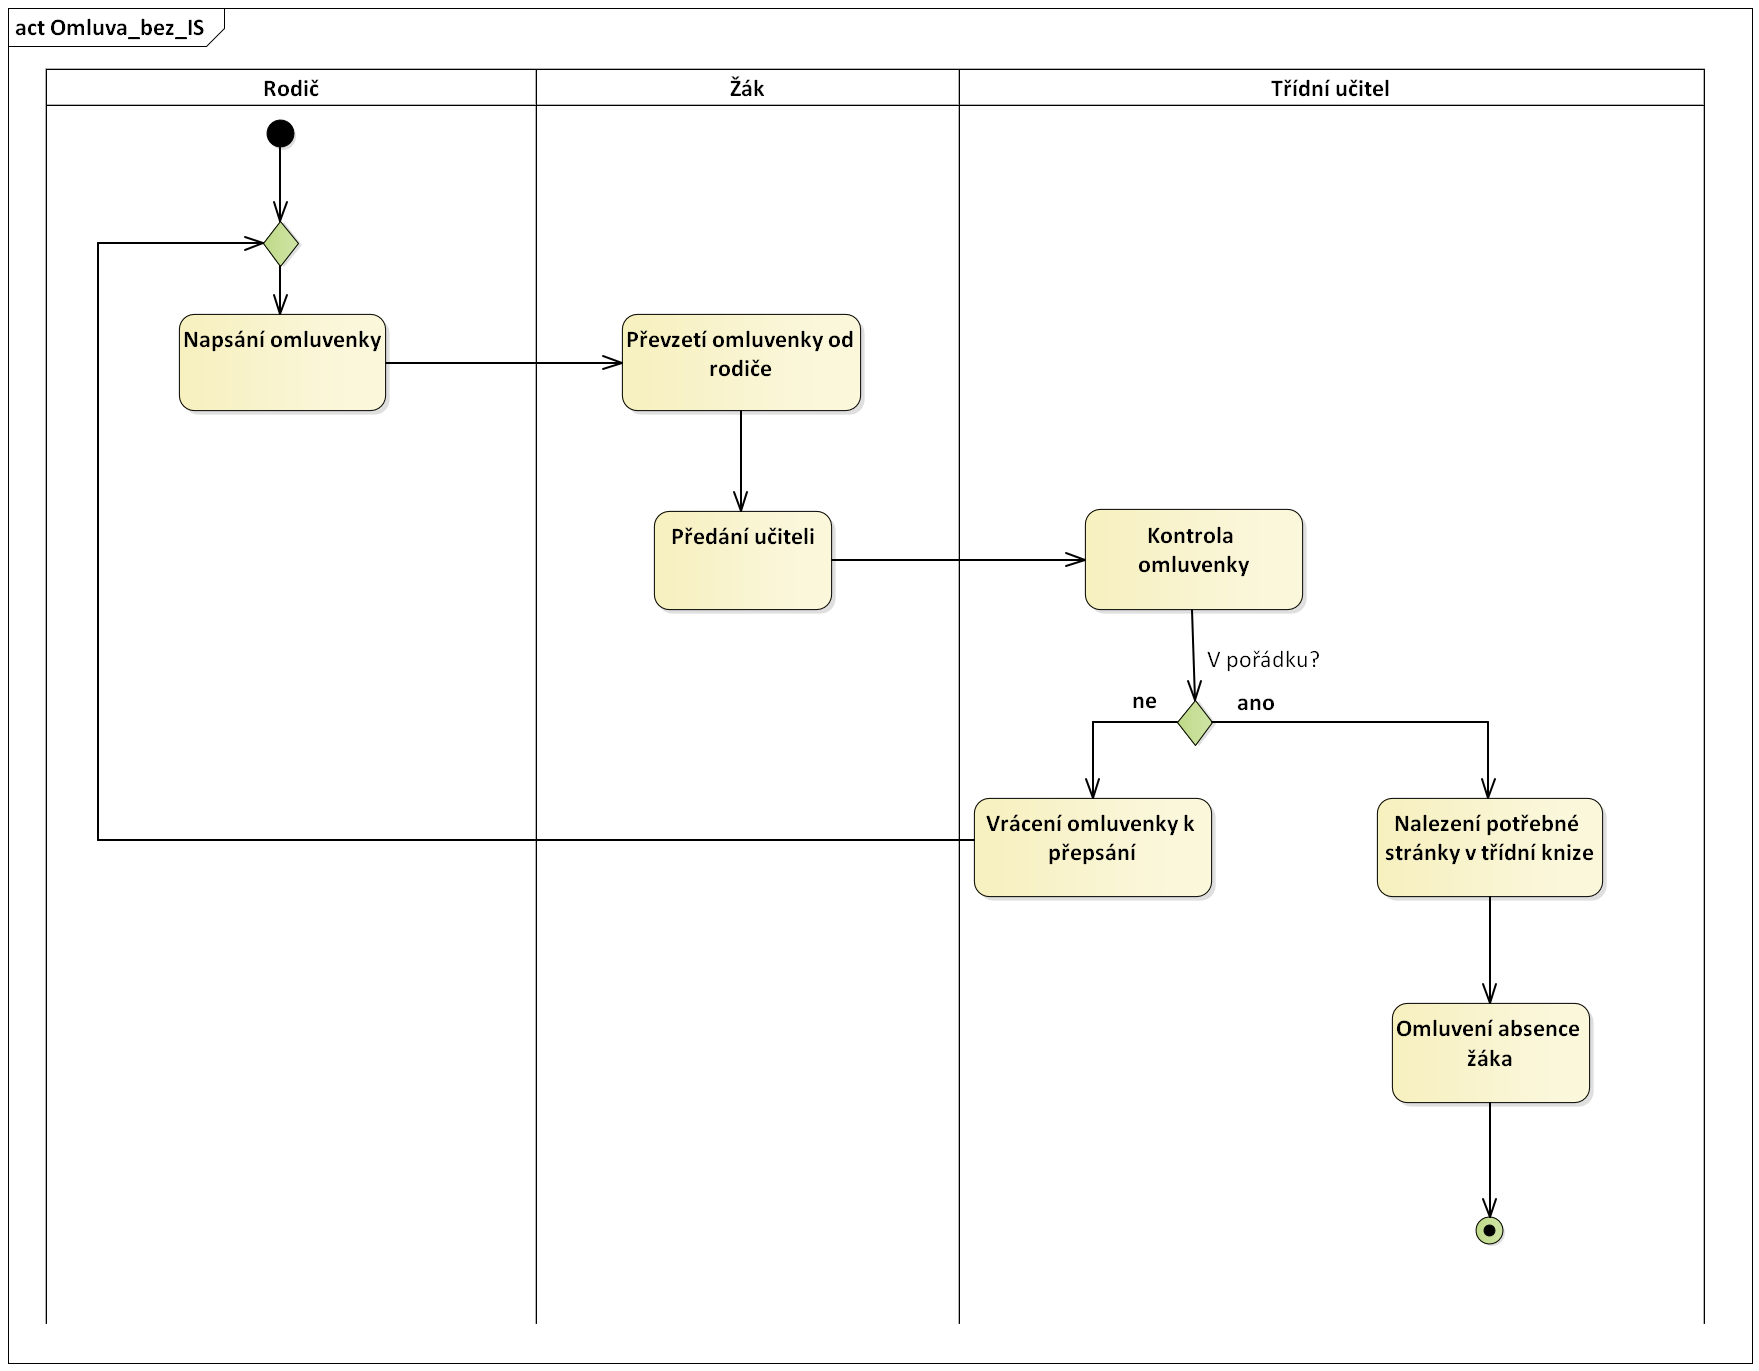
\includegraphics[width=\textwidth]{images/Omluva_bez_IS.png}
	\caption{Proces omlouvání žáků bez informačního systému}
	\label{omluva_bez_IS}
\end{figure}

\subsubsection*{S použitím informačního systému}
Proces s použitím informačního systému začíná opět u rodiče. Po přihlášení rodič vidí upozornění na novou absenci svého dítěte. Přepne se na stránku pro omluvu absencí, napíše zprávu a odešle. V tu chvíli se omluvenka dostává do stavu \uv{odeslána} a třídní učitel dostává upozornění o tom, že někdo poslal omluvenku. Následuje kontrola od třídního učitele. V případě, že je v pořádku, potvrdí omluvenku. Tím se omluvenka dostává do stavu \uv{potvrzena}. Systém poté absenci automaticky omluví a absenci přesune do stavu \uv{omluvená}. Pokud v pořádku není, omluvenku zamítne, čímž se dostává do stavu \uv{zamítnuta}. O zamítnuté omluvence dostane rodič upozornění a proces se opakuje.

Použitím informačního systému se odstranily všechny výše zmiňované problémy. Žák už do tohoto procesu vůbec nezasahuje a nemá tedy možnost omluvenku zfalšovat. Zároveň není možné zamlčet absenci, rodič vždy vidí absence svého dítěte. Vědomé zkracování času vyučování žákem je s použitím informačního systému také vyřešeno.
Tento proces lze vidět namodelovaný na obrázku \ref{omluva_s_IS}.
\clearpage

\begin{figure}[H]
	\centering
	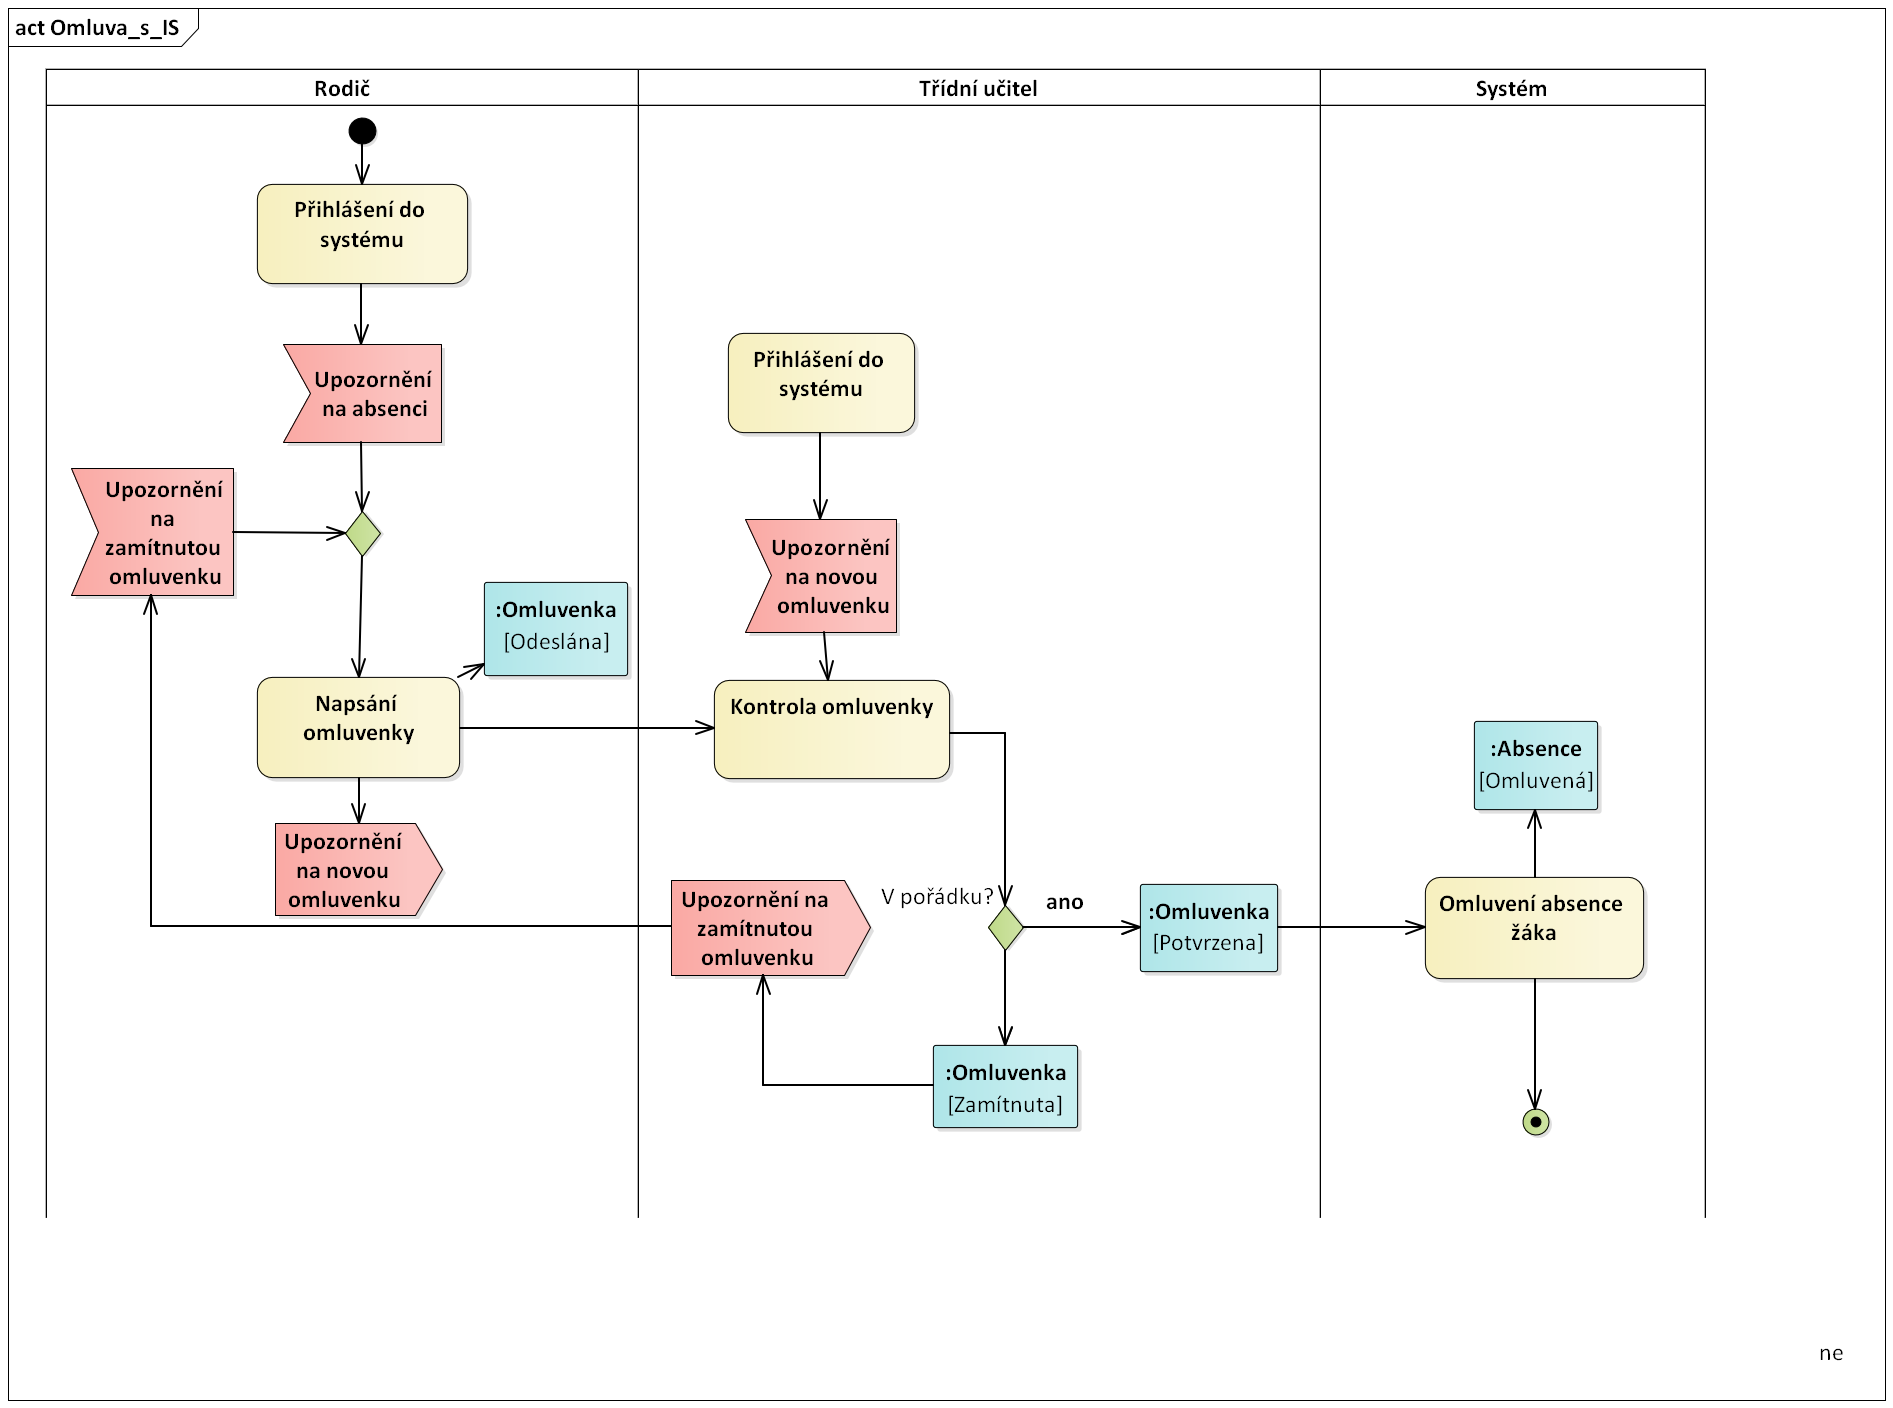
\includegraphics[width=\textwidth]{images/Omluva_s_IS.png}
	\caption{Proces omlouvání žáků s použitím informačního systému}
	\label{omluva_s_IS}
\end{figure}

\subsection{Obecné vytvoření události v hodině}
Zde je nejdříve potřeba si specifikovat, co se myslí událostí v hodině. Událost v hodině je hospitace, suplování, poučení nebo domácí úkol. Událost se vztahuje k určité hodině.
\subsubsection*{Bez použití informačního systému}
Proces je přímočarý. Učitel, zástupce ředitele nebo ředitel nalistuje potřebnou stránku v třídní knize a zapíše záznam o události. Namodelovaný proces je zobrazen na obrázku \ref{udalost_bez_IS}.
\clearpage

\begin{figure}[h]
	\centering
	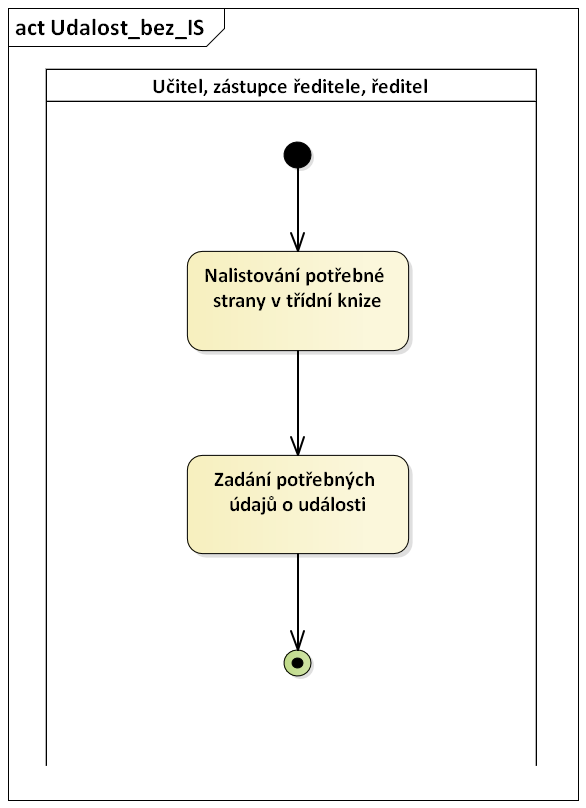
\includegraphics[width=0.5\textwidth]{images/Udalost_bez_IS.png}
	\caption{Proces vytvoření události bez informačního systému}
	\label{udalost_bez_IS}
\end{figure}

\subsubsection*{S použitím informačního systému}
Proces s použitím informačního systému je podobně přímočarý. Uživatel s rolí učitel, zástupce ředitele nebo ředitel se přihlásí do systému, vybere třídní knihu, u zvolené hodiny přidá událost a vyplní potřebné informace.

\subsection{Správa dat}
Tento proces již souvisí se správou dat v nově vytvořeném systému. Nedává smysl uvažovat nad tímto procesem bez informačního systému.

\subsubsection*{S použitím informačního systému}
Proces umožňuje spravovat data o uživatelích, předmětech, třídách, třídních knihách apod. Proces začíná přihlášením uživatele s rolí správce. Ten má možnost přepnout se do administrace systému. Vybere kategorii dat, kterou chce upravovat. Tam má možnost přidávat, odebírat či editovat jednotlivé záznamy.


\section{Doménový model}
Doménový model slouží k vizualizaci objektů reálného světa. Jeho cílem je popsat entity, vztahy mezi nimi a zachytit základní atributy entit. Třídy v doménovém modelu jsou značně zjednodušené a neobsahují žádné metody, pouze důležité atributy.

Doménový model popisující entity a vztahy v systému podporující správu třídních knih je zobrazen na obrázku \ref{domenovy_model}.

\begin{figure}[h]
	\centering
	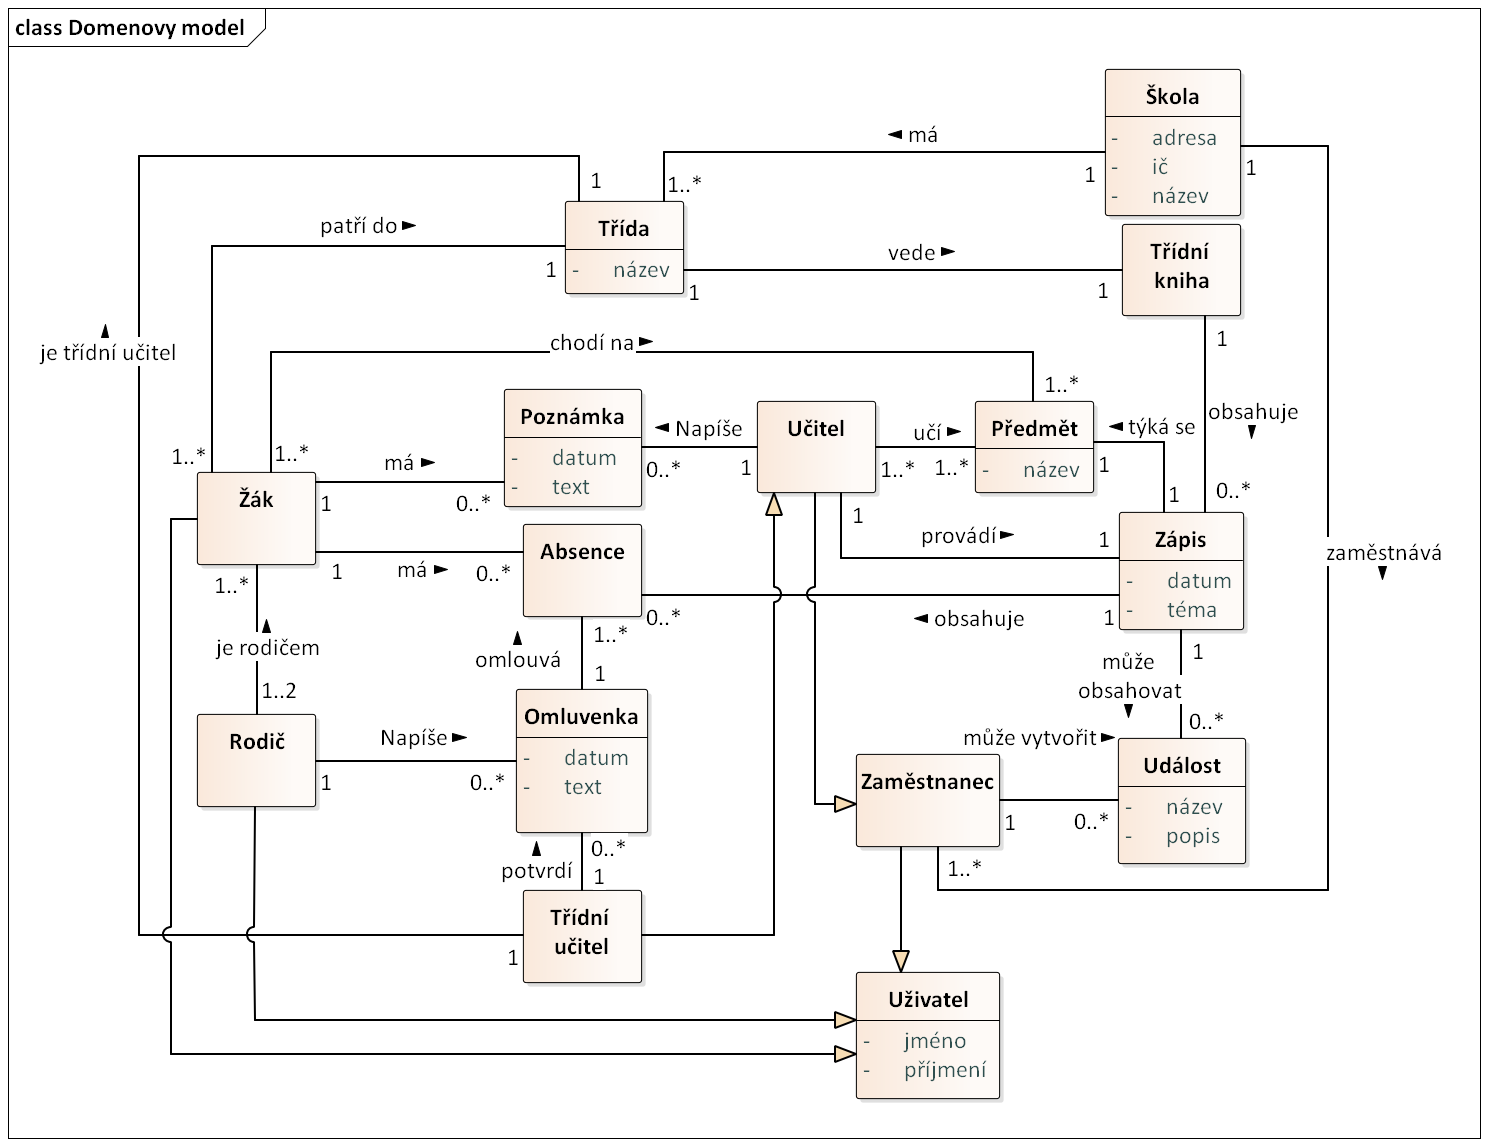
\includegraphics[width=\textwidth]{images/Domenovy_model.png}
	\caption{Doménový model}
	\label{domenovy_model}
\end{figure}

\subsection{Škola}
Třída \texttt{Škola} reprezentuje základní nebo střední školu. Hlavním atributem je název školy, adresa a identifikační číslo osoby (IČO).
\subsection{Třída}
Třída reprezentuje jednotlivé třídy ve škole. \texttt{Třída} má jednoho třídního učitele, jednu třídní knihu a několik žáků.
\subsection{Třídní kniha}
Každá třída je povinna vést třídní knihu. 
\subsection{Zápis}
Třída \texttt{Zápis} reprezentuje jednotlivé zápisy odučených hodin v třídní knize. Zápis se týká určitého předmětu, obsahuje téma a datum. Zápis souvisí s absencemi jednotlivých žáků a může obsahovat událost.
\subsection{Předmět}
Třída \texttt{Předmět} představuje jednotlivé předměty, které se ve škole učí. Předmět může být vyučován více učiteli.
\subsection{Událost}
Tato třída reprezentuje jednotlivé události, které se mohou danou hodinu konat. Jsou to například hospitace, poučení o bezpečnosti, suplování.
\subsection{Poznámka}
Jedná se o jednotlivé poznámky o chování žáků. Poznámku píše učitel určitému žákovi.
\subsection{Absence}
Tato třída představuje absence jednotlivých žáků. Absence musí být omluvena omluvenkou. Absence se vyplňují při zápisu do třídní knihy.

Tato třída má dva stavy. \uv{Neomluvená} a \uv{omluvená}. Při vytvoření absence se automaticky stává neomluvenou absencí. Stavy absence lze vidět na obrázku~\ref{stavy_absence}.

\begin{figure}[h]
	\centering
	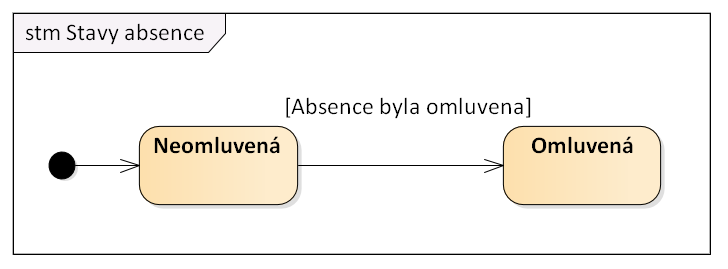
\includegraphics[width=0.75\textwidth]{images/Stavy_absence.png}
	\caption{Stavy absence}
	\label{stavy_absence}
\end{figure}

\subsection{Omluvenka}
Třída představuje omluvenky žáků. Všechny absence žáků musí být řádně omluveny. Omluvenku může napsat pouze rodič (zákonný zástupce) žáka nebo třídní učitel (pokud dostane omluvenku jiným způsobem). Omluvenka napsaná rodičem musí být potvrzena třídním učitelem.

Omluvenka má tři stavy. \uv{Odeslána}, \uv{potvrzena} a \uv{zamítnuta}. Namodelované stavy omluvenky lze vidět na obrázku \ref{stavy_omluvenky}.
\begin{figure}[h]
	\centering
	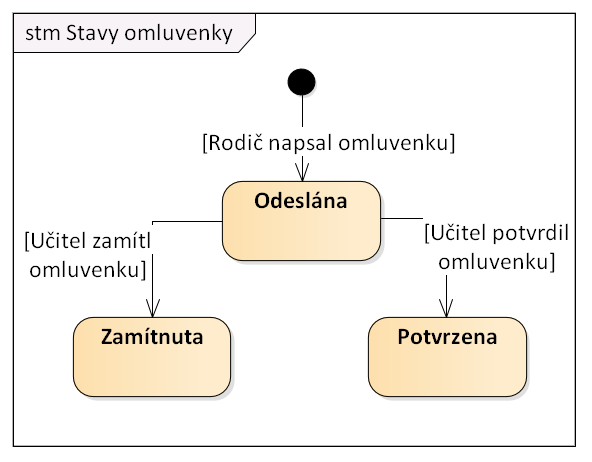
\includegraphics[width=0.6\textwidth]{images/Stavy_omluvenky.png}
	\caption{Stavy omluvenky}
	\label{stavy_omluvenky}
\end{figure}

\subsection{Učitel}
Jednotliví učitelé jsou reprezentováni touto třídou. Učitel je zaměstnán školou, vyučuje určité předměty, zapisuje do třídní knihy a může dávat jednotlivým žákům poznámky o jejich chování.
\subsection{Třídní učitel}
Speciální případ učitele. Má na starosti jednu třídu, u které vykonává činnosti třídního učitele. Jedna z těchto činností je starost o absence jednotlivých žáků. Třídní učitel potvrzuje omluvenky od rodičů žáka a může omluvenku napsat.
\subsection{Rodič}
Tato třída představuje jednoho rodiče (zákonného zástupce) žáka. Rodič může mít ve škole více než jednoho potomka. Žák má minimálně jednoho rodiče, maximálně však dva.
\subsection{Žák}
Třída \texttt{Žák} reprezentuje jednotlivé žáky ve škole, kteří jsou rozděleni do jednotlivých tříd. Žák chodí na určité předměty, může mít absence či poznámky.
\subsection{Zaměstnanec}
\texttt{Zaměstnanec} je nadtřídou pro učitele. Zaměstnanci mohou vytvářet jednotlivé události.
\subsection{Uživatel}
Třída \texttt{Uživatel} je nadtřídou všech možných uživatelů v systému.


\section{Funkční a nefunkční požadavky}
Tato podkapitola je věnována funkčním a nefunkčním požadavkům, které jsou kladeny na výsledný systém. Požadavky byly zpracovány na základě potřeb uživatelů. Tyto potřeby byly konzultovány s Mgr. Lenkou Tichou, která vyučuje na Základní škole Český Dub.

\subsection{Funkční požadavky}
Funkční požadavky jsou požadavky na chování systému. \cite{funkcni_pozadavky}

\subsubsection*{F1 Přihlášení do systému}
Uživatelé se mohou přihlašovat do systému. Registraci nemůže uživatel provést sám, do systému je musí přidat administrátor. Jednotliví uživatelé si mohou změnit heslo. V systému jsou uživatelé rozdělení do jednotlivých rolí:

\begin{itemize}
    \item Správce / administrátor
    \item Ředitel školy
    \item Zástupce ředitele
    \item Třídní učitel
    \item Učitel
    \item Žák
    \item Rodič
\end{itemize}

Jednotlivé role určují uživatelům možnosti, které jim systém poskytne. Jeden uživatel může mít nastaveno více rolí.

\subsubsection*{F2 Správa dat}
Systém bude umožňovat správu dat ve škole. Příkladem dat jsou informace o žácích, učitelích a rodičích, informace o předmětech, které se vyučují, seznam jednotlivých tříd. Tuto správu dat může provádět pouze uživatel s rolí správce.

\subsubsection*{F3 Zápis do třídní knihy}
Systém bude umožňovat uživatelům s rolí učitel zápis do třídní knihy. Učitel zapíše informace o hodině do třídní knihy. Informace, které lze zapsat, jsou absence žáků, předmět, kterého se zápis týká, téma a pořadové číslo hodiny v daný den.

\subsubsection*{F4 Omluva absence žáka}
Systém umožní omlouvat absence žáků. Každá absence žáka musí být řádně omluvena. K omluvení slouží omluvenka, která je napsána rodičem žáka nebo jeho třídním učitelem. V případě, že omluvenku napíše rodič, musí být následně potvrzena třídním učitelem.

\subsubsection*{F5 Vytvoření události v hodině}
V systému bude možné vytvářet v jednotlivých hodinách události. Událostí může být hospitace, suplování, poučení o bezpečnosti nebo domácí úkol. Událost hospitace může vytvořit pouze ředitel nebo zástupce ředitele. Událost domácí úkol a suplování může vytvořit pouze učitel. Poučení může vytvořit libovolný zaměstnanec.

\subsubsection*{F6 Přehledy}
V systému budou zobrazovány přehledy o žácích. Přehledy budou rozděleny podle rolí. 
Uživatel s rolí rodič vidí informace pouze o svých dětech. Žák vidí informace pouze o sobě. Učitelé, zástupce ředitele, ředitel a správci mají přehled o všech žácích.

Zobrazovány budou informace o žákově absenci, poznámkách, případně událostech v hodině (např. domácí úkoly).

\subsubsection*{F7 Archivace dat}
Systém musí umět skladované informace vyexportovat do formátu PDF a vytvořit tak třídní knihu, kterou lze archivovat. V tomto dokumentu musejí být informace o proběhnuté výuce, které byly do systému zapsány v určitém období, typicky za pololetí nebo celý školní rok.
Export do PDF může provádět uživatel s rolí správce, ředitel, zástupce ředitele a třídní učitel.


\subsection{Nefunkční požadavky}
Nefunkční požadavky určují omezení, která jsou kladena na systém. 
\subsubsection*{N1 Webová aplikace}
Systém bude vytvořen jako webová aplikace. Aplikace bude plně funkční pro webový prohlížeč Google Chrome 87.0.4280.88. 

\subsubsection*{N2 Responzivní design}
Design webové stránky bude responzivní, bude se přizpůsobovat velikosti okna, případně používanému zařízení.

\subsubsection*{N3 Snadná rozšiřitelnost systému}
Architektura systému bude navržena tak, aby případné budoucí rozšíření systému bylo co nejjednodušší.

